\documentclass[11pt]{article}
\usepackage[utf8]{inputenc}
\usepackage[T1]{fontenc}
\usepackage{amsmath, amssymb}
\usepackage{graphicx}
\usepackage[a4paper, margin=1in]{geometry}
\usepackage{hyperref}
\usepackage{booktabs}
\usepackage{tabularx}
\usepackage{xcolor}

\hypersetup{
    colorlinks=true,
    linkcolor=blue,
    filecolor=magenta,      
    urlcolor=cyan,
    pdftitle={Generalized Reversible Computation Summary},
    pdfauthor={Canonical}
}

\title{Generalized Reversible Computation (GRC): A New Paradigm for Unifying Software Construction and Evolution (Summary)}
\author{Canonical \\ \texttt{canonical\_entropy@163.com}}
\date{\today}

\begin{document}

\maketitle

\section{Core Concepts and Formula}

Traditional software engineering faces fundamental contradictions between standardization and customization, reuse and evolution, entropy increase and control. The \textbf{Generalized Reversible Computation (GRC)} proposed in this paper aims to resolve these contradictions through a unified theoretical framework.

The core idea of GRC is to extend the principle of "reversibility" from logical reversibility at \textbf{runtime} to construction reversibility at \textbf{build-time} throughout the entire software lifecycle. Its foundation is a unified construction formula:

\[
\text{App} = \text{Generator}\langle\text{DSL}\rangle \oplus \Delta
\]

Where:
\begin{itemize}
    \item \textbf{App}: The final software application.
    \item \textbf{Generator$\langle$DSL$\rangle$}: \textbf{Predictable ideal backbone}. A deterministic generator reads Domain-Specific Language (DSL) descriptions to build a standardized, idealized foundation for the system.
    \item \textbf{$\Delta$ (Structured Delta)}: \textbf{Perturbation term encapsulating all changes}. It is a structured data packet recording all customized and evolutionary modifications (additions, deletions, changes) on the base model.
    \item \textbf{$\oplus$ (Reversible merge operator)}: An algebraic operation that applies the delta $\Delta$ non-intrusively to the base model, theoretically supporting inverse operations.
\end{itemize}

The ultimate goal of GRC is: \textbf{to elevate software construction from an irreversible instructional process to a solvable algebraic equation.}

\section{Theoretical Foundation and Positioning}

\begin{itemize}
    \item \textbf{Analogy with Physics}: GRC's methodology is similar to the \textbf{Dirac picture (interaction picture)} in quantum mechanics. It decomposes a complex system into an "exactly solvable" free part (Generator$\langle$DSL$\rangle$) and an interaction part treated as a "perturbation" ($\Delta$). This makes GRC a computational framework focused on \textbf{managing complexity}.
    \item \textbf{Principle of Minimum Information Expression}: This is the first principle of GRC. It requires that software artifacts contain only the complexity necessary to solve the specific problem. This naturally leads to three strategies:
    \begin{enumerate}
        \item Use \textbf{declarative DSLs} to minimize accidental complexity related to technical implementation.
        \item Pursue \textbf{semantic uniqueness and reversible transformations}, ensuring lossless conversion of core semantics across different forms of expression.
        \item Use \textbf{delta ($\Delta$) as the minimal unit of evolution}, most economically describing system changes.
    \end{enumerate}
\end{itemize}

\section{Core Mechanisms}

\subsection{Recursive Fractal-like Construction}
The GRC construction formula \( Y = F(X) \oplus \Delta \) exhibits \textbf{self-similarity} at all levels:
\begin{itemize}
    \item \textbf{Vertical Recursion}: Building multi-stage software pipelines (e.g., XMeta $\leftarrow$ XORM $\leftarrow$ Excel), where each stage follows the "generation + delta" pattern.
    \item \textbf{Horizontal Recursion}: An application is composed of multiple DSL models and their deltas.
    \item \textbf{Temporal Recursion}: System version evolution is a process of delta superposition (\( V_2 = V_1 \oplus \Delta \)).
    \item \textbf{Meta-recursion}: The construction system itself (generators, DSL definitions) also evolves according to this pattern.
\end{itemize}

\subsection{Delta Algebra}
The mathematical core of GRC is \textbf{delta algebra}. It introduces an \textbf{inverse element ($-\Delta$)} for the merge operator $\oplus$, enabling:
\begin{itemize}
    \item \textbf{Precise Delta Calculation}: $\Delta = \text{App} - \text{Base}$ (Semantic diff)
    \item \textbf{Safe Stripping of Changes}: $\text{Base} = \text{App} - \Delta$ (Semantic rebase)
\end{itemize}
This achieves a paradigm shift from "reusing what is identical" to "\textbf{reusing what is related}."

\subsection{Three Dimensions of Reversibility}
Reversibility in GRC is a multi-dimensional engineering principle:
\begin{itemize}
    \item \textbf{Algebraic Reversibility}: The construction process is a solvable algebraic equation, supporting the calculation and stripping of deltas.
    \item \textbf{Transformational Reversibility}: Establishes high-fidelity "semantic round-tripping" between different forms of expression (DSL, code, GUI, Excel), ensuring lossless information flow.
    \item \textbf{Process Reversibility}: Allows non-intrusive correction and compensation of already released systems using future deltas $\Delta$, breaking the linear causality of the physical world.
\end{itemize}

\section{Unifying Explanatory Power and Practical Validation}

\subsection{Reinterpreting Domain-Driven Design}
GRC provides a new theoretical perspective for DDD, proposing that the \textbf{core role of an Aggregate Root is to be the carrier of the domain language and a unified map for information access}. Based on the principle of "separating structure (data) from dynamics (process)":
\begin{itemize}
    \item \textbf{Data Aggregate}: A pure information space providing a unified view rich in domain semantics.
    \item \textbf{Behavior Aggregate}: A process orchestrator described by a DSL, decomposing complex logic into a series of composable steps.
\end{itemize}
Domain events are viewed as deltas in the state space ($\text{NewState} = \text{OldState} \oplus \text{Event}$), and software evolution is the application of deltas within the coordinate system defined by the DSL.

\subsection{Unifying Modern Technical Practices}
GRC reveals that modern technologies like Docker, Kustomize, and Pixar's OpenUSD have independently "rediscovered" the delta-first construction logic, forming evidence of "convergent evolution."
\begin{itemize}
    \item \textbf{Docker}: Image layers are deltas ($\Delta$) in the \textbf{filesystem structure space}, and OverlayFS is the merge operator ($\oplus$).
    \item \textbf{OpenUSD}: `.usd` files act as delta layers ($\Delta$) that are non-destructively superimposed in the 3D scene graph space.
\end{itemize}

\subsection{Case Validation: Nop Platform and Banking System Refactoring}
The GRC theory is validated through the \textbf{Nop Platform} (its canonical implementation) and a refactoring case of a large-scale banking core system.

\begin{itemize}
    \item \textbf{Nop Platform}: Implements the GRC formula based on a unified `XNode` metamodel and the `XLang` language system. Its core engineering pillars include:
    \begin{itemize}
        \item \textbf{"Loader as Generator"}: Introduces delta merging capability non-intrusively by intercepting the configuration loading process of standard frameworks (like Spring), transforming load-time into a construction phase.
        \item \textbf{XDef Metamodel}: Defines new DSLs at O(1) marginal cost and automatically gains full GRC toolchain support (parsing, validation, IDE support, delta merging).
        \item \textbf{S-N-V Three-Stage Loading}: A rigorous engineering implementation of "phase separation" that confines all complexity to the controlled \textbf{load-time}, ensuring runtime purity and efficiency:
        \begin{itemize}
            \item \textbf{S (Source/Structure Merge)}: All source files (DSLs) are parsed into a unified `XNode` intermediate representation. Delta merging (`x-extends`) and metaprogramming (Xpl template execution) occur \textbf{exclusively} in this unified structural space, producing a "coarse" but structurally complete model tree.
            \item \textbf{N (Node/Normalization)}: Domain-specific semantic processing occurs, including default value application, derived property calculation, and shorthand syntax expansion, resulting in a semantically rich "refined" model tree.
            \item \textbf{V (View/Validation)}: The normalized model is compiled into immutable, strongly-typed runtime objects (the \textbf{View}), followed by final validation. The output is a pure, high-performance static model for runtime execution.
        \end{itemize}
        This process ensures that all GRC "magic" (delta merging, code generation) completes during loading, while the runtime operates on pre-"baked" static models, eliminating debugging complexity and ensuring deterministic construction.
    \end{itemize}
    
    \begin{figure}[htbp]
        \centering
        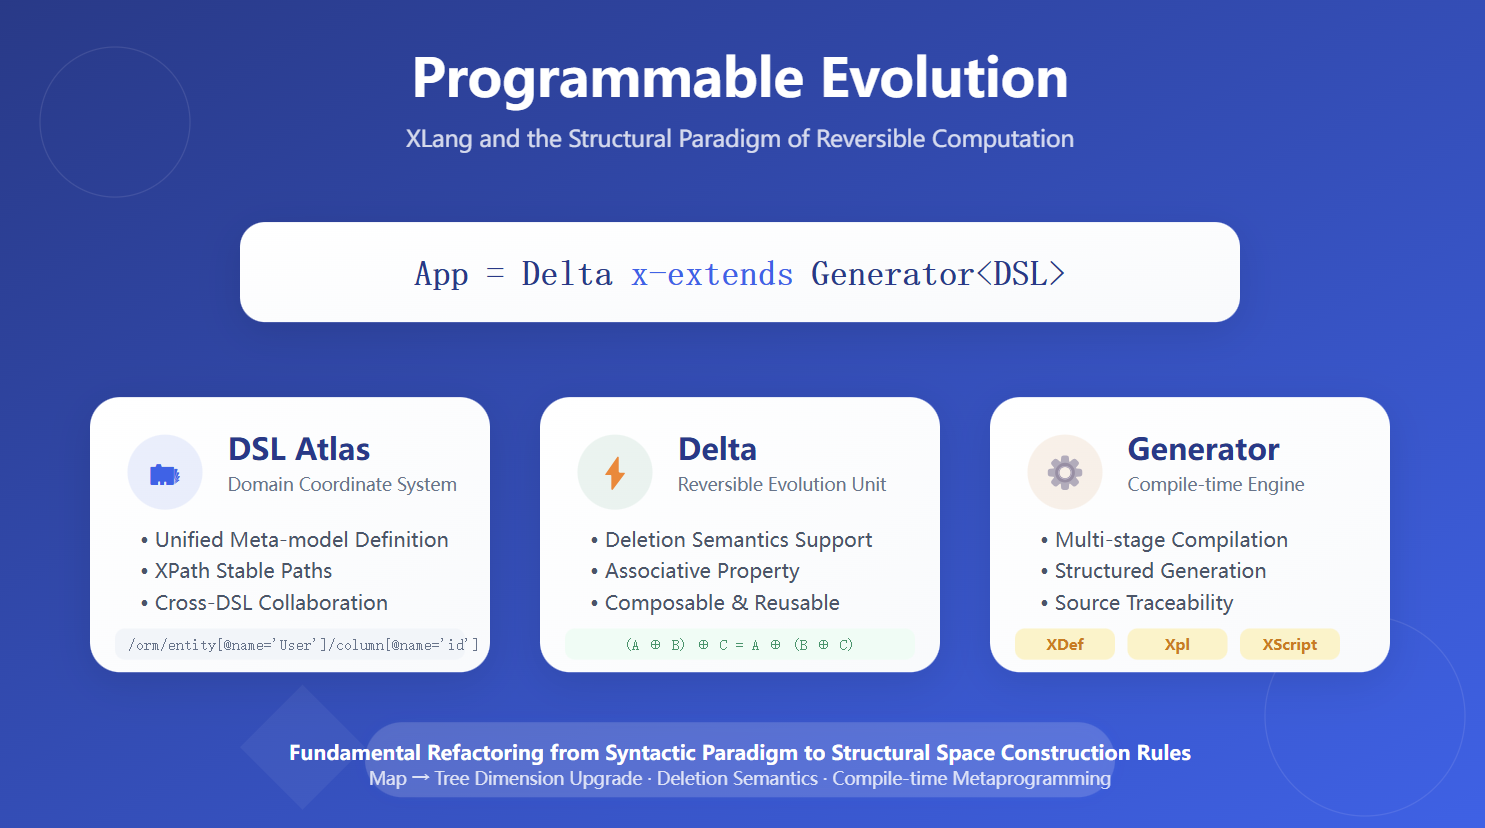
\includegraphics[width=0.9\textwidth]{ddd/xlang-paradigm.png} 
        \caption{The XLang Implementation of the GRC Paradigm}
        \label{fig:xlang_paradigm}
    \end{figure}
    
    \item \textbf{Banking Case}: Refactored a complex "order placement" process from a traditional "God Aggregate Root" into a combination of a \textbf{DSL-declared process} (behavior aggregate) and \textbf{pure data objects} (data aggregate). For customization needs of different clients, there was no need to modify the core code; simply providing a declarative delta YAML file ($\Delta$) and using the `x:extends` mechanism achieved non-intrusive customization, perfectly resolving the core conflict between standardized products and client customizations.
\end{itemize}

\section{Conclusion and Outlook}

Generalized Reversible Computation (GRC) provides a systematic, scalable, and theoretically sound new paradigm for unifying software construction and evolution by elevating the \textbf{structured delta ($\Delta$)} to a computable and composable first-class citizen. Its core formula $\text{App} = \text{Generator}\langle\text{DSL}\rangle \oplus \Delta$ and its recursive fractal properties offer us a new perspective and methodology for managing software complexity and coping with continuous evolution.

Future work includes further formalization of delta algebra, exploring the integration of AI and GRC, optimizing the developer experience, and validating applications in broader domains. GRC has the potential to evolve from a novel theoretical paradigm into a mature infrastructure that profoundly changes the way software is produced.

\end{document}